\mfpicnumber{1}

\opengraphsfile{IntrotoConics}

\setcounter{footnote}{0}

\label{IntrotoConics}

In this chapter, we study the \index{conic sections ! definition} \textbf{Conic Sections} - literally `sections of a  cone'.  Imagine a double-napped cone as seen below being `sliced' by a plane. 

\centerline{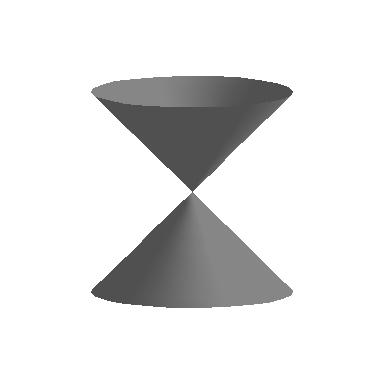
\includegraphics[width=2in]{./ConicsGraphics/cone.jpg}}

If we slice the cone with a horizontal plane the resulting curve is a \index{circle ! from slicing a cone} \textbf{circle}.

\begin{center}

\begin{tabular}{cc}

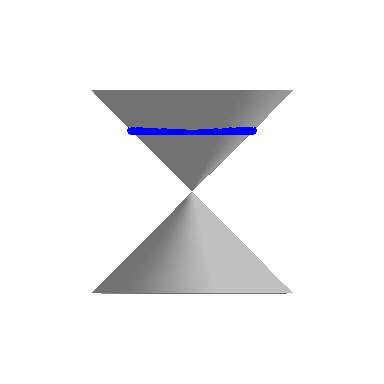
\includegraphics[width=2in]{./ConicsGraphics/Circle01.jpg} & 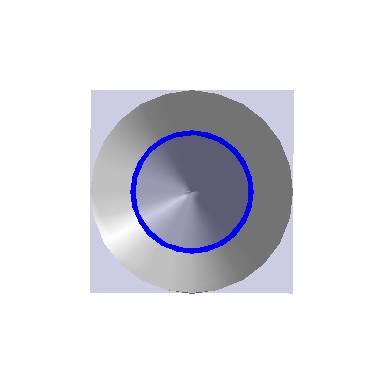
\includegraphics[width=2in]{./ConicsGraphics/Circle02.jpg} \\

\end{tabular}

\end{center}

\pagebreak

Tilting the plane ever so slightly produces an \index{ellipse ! from slicing a cone} \textbf{ellipse}.

\begin{center}

\begin{tabular}{cc}

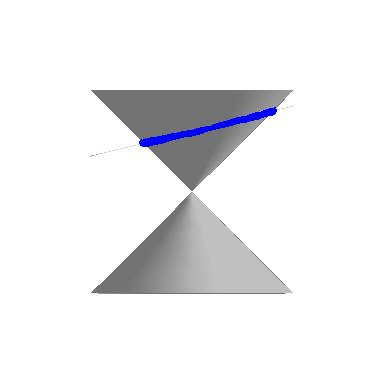
\includegraphics[width=2in]{./ConicsGraphics/Ellipse01.jpg} & 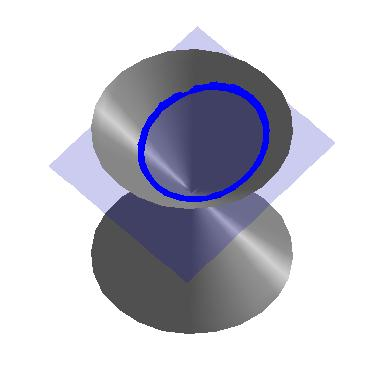
\includegraphics[width=2in]{./ConicsGraphics/Ellipse02.jpg} \\

\end{tabular}

\end{center}

If the plane cuts parallel to the cone, we get a \index{parabola ! from slicing a cone} \textbf{parabola}.

\begin{center}

\begin{tabular}{cc}

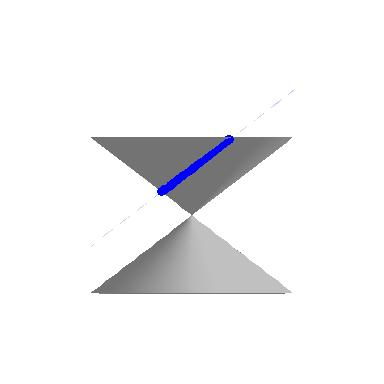
\includegraphics[width=2in]{./ConicsGraphics/Parabola01.jpg} & 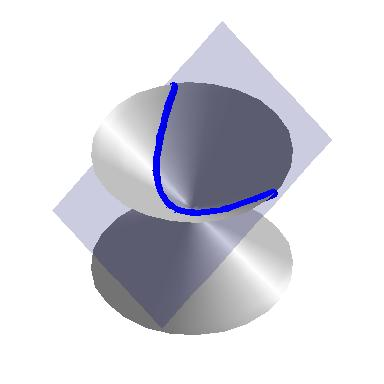
\includegraphics[width=2in]{./ConicsGraphics/Parabola02.jpg} \\

\end{tabular}

\end{center}

If we slice the cone with a vertical plane, we get a \index{hyperbola ! from slicing a cone} \textbf{hyperbola}.

\begin{center}

\begin{tabular}{cc}

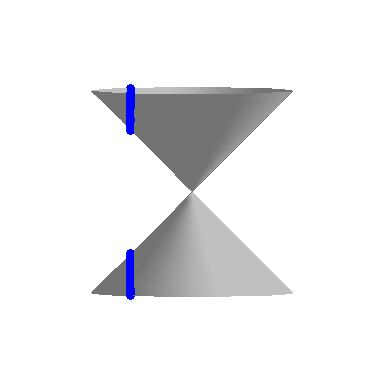
\includegraphics[width=2in]{./ConicsGraphics/Hyperbola01.jpg} & 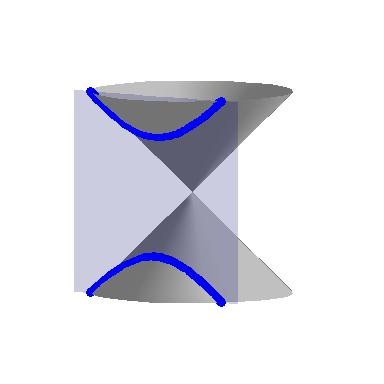
\includegraphics[width=2in]{./ConicsGraphics/Hyperbola02.jpg} \\

\end{tabular}

\end{center}

For a wonderful animation describing the conics as intersections of planes and cones, see Dr. Louis Talman's  \href{http://clem.mscd.edu/~talmanl/HTML/ConicSections.html}{\underline{Mathematics Animated Website}}.

\pagebreak

If the slicing plane contains the vertex of the cone, we get the so-called `degenerate' conics:  a point, a line, or two intersecting lines.  

\phantomsection
\label{degenerateconics}

\begin{center}

\begin{tabular}{cc}

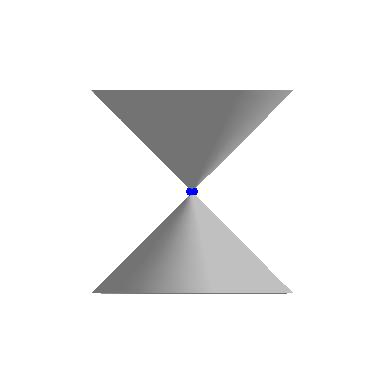
\includegraphics[width=2in]{./ConicsGraphics/Point01.jpg} & 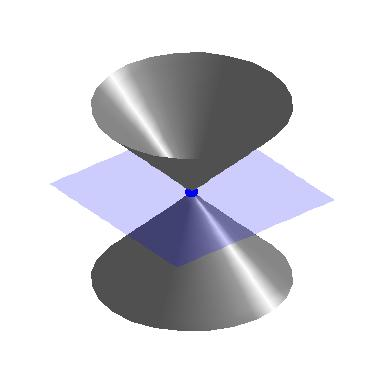
\includegraphics[width=2in]{./ConicsGraphics/Point02.jpg} \\


\includegraphics[width=2in]{./ConicsGraphics/Ilines01.jpg} & 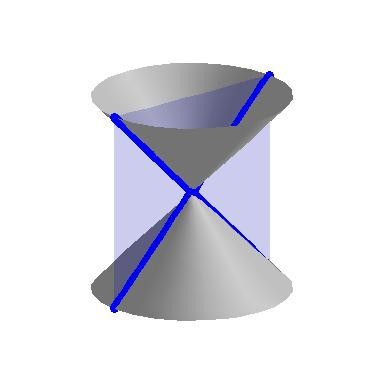
\includegraphics[width=2in]{./ConicsGraphics/Ilines02.jpg}\\

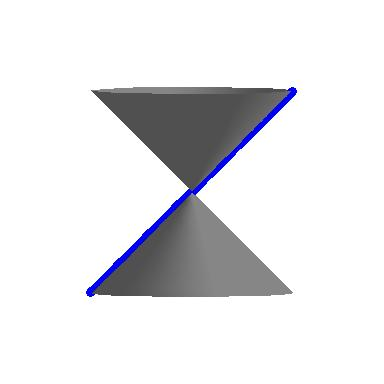
\includegraphics[width=2in]{./ConicsGraphics/Tline01.jpg} & 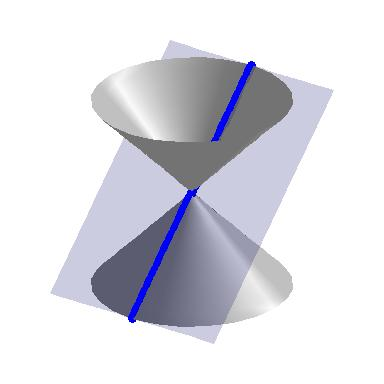
\includegraphics[width=2in]{./ConicsGraphics/Tline02.jpg} \\

\end{tabular}

\end{center}


We will focus the discussion on the non-degenerate cases:  circles, parabolas, ellipses, and hyperbolas, in that order. To determine equations which describe these curves, we will make use of their definitions in terms of distances. 

\closegraphsfile